% Algorithm Diagram
\resizebox{\textwidth}{!}{
\begin{tikzpicture}[roundnode/.style={circle, draw=green!60, fill=green!5, very
thick, minimum size=7mm}, squarenode/.style={rectangle, draw=red!60, fill=red!5,
very thick, minimum size=5mm},
]
    \node[squarenode](start) {START};
    \node[roundnode](database) [right=of start] {\begin{tikzpicture}
        \draw[thin] (0,0) rectangle (5,4);
        \draw[thin] (0, 0.5) -- (5, 0.5);
        \draw[thin] (0, 1) -- (5, 1);
        \draw[thin] (0, 1.5) -- (5, 1.5);
        \draw[thin] (0, 2) -- (5, 2);
        \draw[thin] (0, 2.5) -- (5, 2.5);
        \draw[thin] (0, 3) -- (5, 3);
        \draw[thin] (0, 3.5) -- (5, 3.5);
        \draw[thin] (1, 0) -- (1, 4);
        \draw[thin] (2, 0) -- (2, 4);
        \draw[thin] (3, 0) -- (3, 4);
        \draw[thin] (4, 0) -- (4, 4);
        \node[above] at (0, 4) {\small create the database};
    \end{tikzpicture}};
    \node[squarenode](while) [right=of database] {THEN WHILE NOT STOPPED};
    \node[roundnode](select_strat) [below=of while] {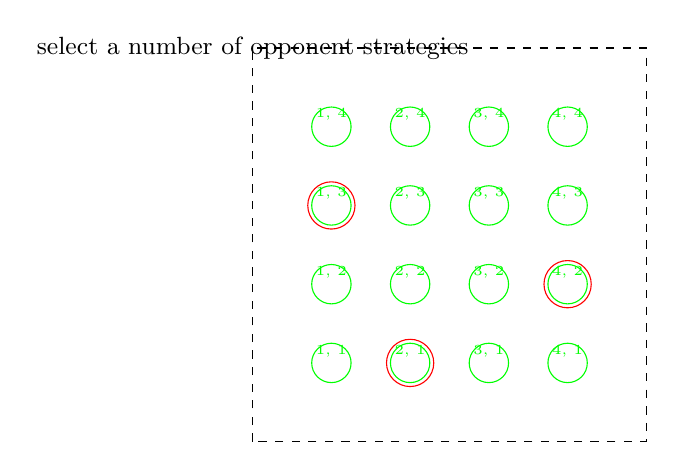
\begin{tikzpicture}
        \draw[thin, dashed] (0, 0) rectangle (5, 5);
        \foreach \x in {1, 2, 3, 4}
            \foreach \y in {1, 2, 3, 4}
                {\draw[green] (\x, \y) circle (0.25);
                \node[green, below] at (\x, \y + 0.35) {\tiny \x, \y};}
        \node at (0, 5) {\small select a number of opponent strategies};
        \draw[red] (1, 3) circle (0.3);
        \draw[red] (2, 1) circle (0.3);
        \draw[red] (4, 2) circle (0.3);
    \end{tikzpicture}};
    \node[roundnode](defector) [left=of select_strat] {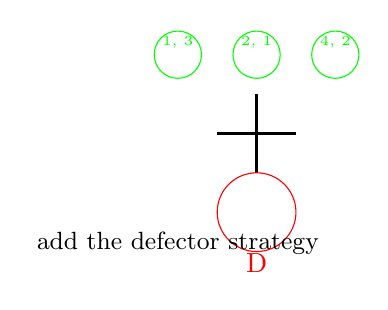
\begin{tikzpicture}
        \draw[green] (0, 0) circle (0.3);
        \node[green, below] at (0, 0.35) {\tiny 1, 3};
        \draw[green] (1, 0) circle (0.3);
        \node[green, below] at (1, 0.35) {\tiny 2, 1};
        \draw[green] (2, 0) circle (0.3);
        \node[green, below] at (2, 0.35) {\tiny 4, 2};
        \draw[thick] (0.5, -1) -- (1.5, -1);
        \draw[thick] (1, -1.5) -- (1, -0.5);
        \draw[red] (1, -2) circle (0.5);
        \node[red, below] at (1, -2.4) {D};
        \node at (0, -2.4) {\small add the defector strategy};
    \end{tikzpicture}};
    \node[squarenode](noise&probs) [left=of defector] {FOR EVERY $p_{n}$ AND $p_{e}$};
    \node[roundnode](tournament) [below=of noise&probs] {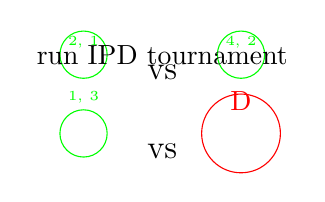
\begin{tikzpicture}
        \draw[green] (0,0) circle (0.3);
        \node[green, below] at (0, 0.35) {\tiny 2, 1};
        \node[thick, below] at (1, 0) {\large vs};
        \draw[green] (2, 0) circle (0.3);
        \node[green, below] at (2, 0.35) {\tiny 4, 2};
        \draw[green] (0, -1) circle (0.3);
        \node[green, below] at (0, -0.35) {\tiny 1, 3};
        \node[thick, below] at (1, -1) {\large vs};
        \draw[red] (2, -1) circle (0.5);
        \node[red, below] at (2, -0.35) {D};
        \node at (1, 0) {run IPD tournament};
    \end{tikzpicture}};
    \node[roundnode](payoffs) [right=of tournament] {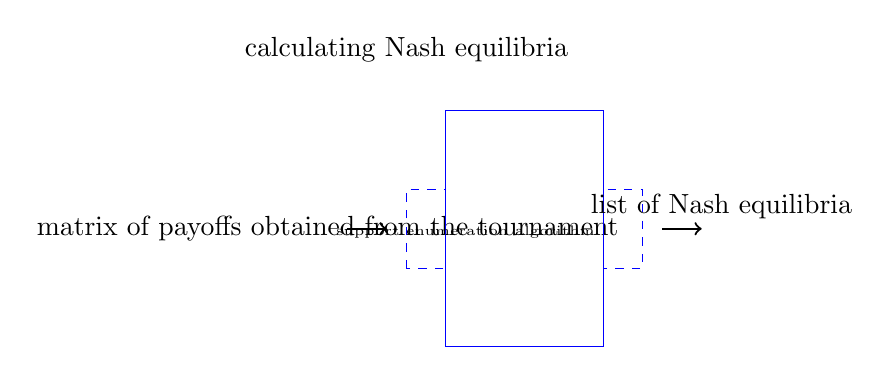
\begin{tikzpicture}
        \node at (0, 0) {matrix of payoffs obtained from the
        tournament};
        \draw[->, thick] (0.25, 0) -- (0.75, 0);
        \draw[blue, dashed] (1, -0.5) rectangle (1.5, 0.5);
        \draw[blue] (1.5, -1.5) rectangle (3.5, 1.5);
        \draw[blue, dashed] (3.5, -0.5) rectangle (4, 0.5);
        \draw[->, thick] (4.25, 0) -- (4.75, 0);
        \node[above] at (5, 0) {list of Nash equilibria};
        \node[above] at (1, 2) {calculating Nash equilibria};
        \node[above] at (1.75, -0.25) {\tiny support enumeration algorithm};
    \end{tikzpicture}};
    \node[squarenode](writing) [right=of payoffs] {WRITE RESULTS TO DATABASE};

    \draw[->] (start.east) -- (database.west);
    \draw[->] (database.east) -- (while.west);
    \draw[->] (while.south) -- (select_strat.north);
    \draw[->] (select_strat.west) -- (defector.east);
    \draw[->] (defector.west) -- (noise&probs.east);
    \draw[->] (noise&probs.south) -- (tournament.north);
    \draw[->] (tournament.east) -- (payoffs.west);
    \draw[->] (payoffs.east) -- (writing.west);
    \draw[->] (writing.west) .. controls +(right:2) and +(up:2) .. (while.west);
\end{tikzpicture}
}